\documentclass[12pt, a4paper]{article}

%% ─── Packages ────────────────────────────────────────────────────────────────
\usepackage[T1]{fontenc}
\usepackage[utf8]{inputenc}
\usepackage{geometry}
\usepackage{graphicx}
\usepackage{booktabs}
\usepackage{longtable}
\usepackage{array}
\usepackage{multirow}
\usepackage{amsmath}
\usepackage{amssymb}
\usepackage{mathtools}
\usepackage{stmaryrd}
\usepackage{hyperref}
\usepackage{xcolor}
\usepackage{setspace}
\usepackage{caption}
\usepackage{float}
\usepackage{enumitem}
\usepackage{titlesec}
\usepackage{fancyhdr}
\usepackage{parskip}

%% ─── Page geometry ───────────────────────────────────────────────────────────
\geometry{
  a4paper,
  top=2.5cm, bottom=2.5cm,
  left=2.5cm, right=2.5cm,
  headheight=15pt
}

%% ─── Header / footer ─────────────────────────────────────────────────────────
\pagestyle{fancy}
\fancyhf{}
\renewcommand{\headrulewidth}{0.4pt}
\fancyhead[L]{\small Enquête Nationale sur l'Emploi -- Composante Ménages}
\fancyhead[R]{\small Note Méthodologique -- Octobre 2024}
\fancyfoot[C]{\thepage}

%% ─── Section formatting ──────────────────────────────────────────────────────
\titleformat{\section}{\large\bfseries}{}{0em}{}[\titlerule]
\titleformat{\subsection}{\normalsize\bfseries}{}{0em}{}
\titleformat{\subsubsection}{\normalsize\itshape\bfseries}{}{0em}{}

%% ─── Hyperref ────────────────────────────────────────────────────────────────
\hypersetup{
  colorlinks=true,
  linkcolor=blue!60!black,
  urlcolor=blue!60!black,
  citecolor=blue!60!black
}

%% ─── Custom column type ──────────────────────────────────────────────────────
\newcolumntype{P}[1]{>{\centering\arraybackslash}p{#1}}

%% ─── Document ────────────────────────────────────────────────────────────────
\begin{document}

%% ─── Title page ──────────────────────────────────────────────────────────────
\thispagestyle{empty}
\begin{center}
  \vspace*{1cm}
  \includegraphics[width=7cm]{image1.png}\\[1.5cm]
  {\LARGE\bfseries Agence Nationale de la Statistique}\\[0.4cm]
  \rule{\textwidth}{1pt}\\[0.6cm]
  {\Large\bfseries Enquête Nationale sur l'Emploi :}\\[0.3cm]
  {\Large\bfseries Composante Ménages}\\[0.6cm]
  \rule{\textwidth}{1pt}\\[0.8cm]
  {\large\bfseries Note méthodologique}\\[0.5cm]
  {\large Octobre 2024}
  \vfill
\end{center}
\newpage

\setcounter{page}{1}
\tableofcontents
\newpage

%% ─── Introduction ────────────────────────────────────────────────────────────
\section{Introduction}

L'analyse de l'emploi est une composante importante de la dynamique de l'économie d'une nation. Elle est également d'un intérêt majeur pour le gouvernement ivoirien qui l'a intégré dans les différents Plans Nationaux de Développement (PND, 2012--2015 et 2016--2020).

La mesure de l'emploi est affectée aux instituts (agences) nationaux (nationales) de statistique qui mettent en \oe{}uvre des processus de collecte et d'analyse des données sur l'emploi à l'échelle nationale. En ce sens, le gouvernement a adopté en 2012 la réalisation d'une enquête annuelle sur l'emploi. Cette volonté a donné naissance en premier à l'Enquête Nationale sur la Situation de l'Emploi et du Travail des Enfants (ENSETE) en 2013 et s'est par la suite déclinée à travers l'Enquête Nationale sur la Situation de l'Emploi et du Secteur Informel (ENSESI) en 2016, l'Enquête Régionale Intégrée sur l'Emploi et le Secteur Informel (ERI-ESI) en 2017 et l'Enquête Nationale sur l'Emploi (ENE) en 2019.

L'analyse de l'emploi est régie par les normes internationales de la Conférence Internationale des Statisticiens du Travail (CIST). Dans ce sens, les trois dernières enquêtes emploi, à savoir l'ENE, l'ERI-ESI et l'ENSESI, ont été réalisées en intégrant les normes et recommandations de la 19\textsuperscript{ème} CIST tenu en 2013. Toutefois, une meilleure conformité aux exigences de la CIST nécessite des efforts supplémentaires de la part du système statistique ivoirien.

Il est, en effet, recommandé par la CIST, la production plusieurs fois par an d'indicateurs sur les principales grandeurs de l'emploi, la main-d'\oe{}uvre et du chômage dans le but de surveiller les variations saisonnières (trimestrielles, semestrielles ou mensuelles). Il est également recommandé la production de statistiques annuelles sur la main-d'\oe{}uvre, la sous-utilisation de la main-d'\oe{}uvre, le chômage et une analyse structurelle des marchés et des statistiques sur le temps de travail. Enfin, des analyses macro et micro économiques approfondies sont attendues afin d'orienter les politiques publiques sur des sujets socio-économiques.

Dans la volonté de pallier ce gap entre le système de collecte de données actuel sur l'emploi et les normes et recommandations de la CIST, l'Agence Nationale de la Statistique de Côte d'Ivoire a initié une réforme de son appareil de collecte de données sur l'emploi. Cette réforme permettra une analyse plus approfondie de l'emploi en Côte d'Ivoire en mettant en évidence la situation de l'offre d'emploi et de la demande d'emploi.

La présente note méthodologique propose une réforme du processus de collecte de données sur la demande d'emploi en Côte d'Ivoire. Cette proposition prend la forme d'une nouvelle enquête emploi, l'Enquête Nationale sur l'Emploi auprès des ménages (ENE-M). Cette enquête sera réalisée en continue tout au long de l'année et portera sur chacune des semaines de l'année. Elle permettra de mesurer les différents indicateurs de aussi bien trimestriellement qu'annuellement. Elle permettra des analyses plus approfondies de certaines thématiques liées à l'emploi telles la santé, l'éducation, etc.

La Figure~\ref{fig:cycle_production} présente le cycle complet de production de l'ENE-M, de la collecte des données jusqu'à la diffusion des résultats. Ce cycle s'étend sur deux trimestres consécutifs : les données du trimestre $T$ sont collectées en continu, puis consolidées, pondérées et analysées au cours du trimestre $T+1$, pour une publication finale respectant la date butoir de 90 jours après la fin du trimestre de référence. L'ensemble des phases de traitement statistique — apurement, pondération, calage et génération des sorties — est automatisé selon l'approche des Pipelines Analytiques Reproductibles (RAP).

\begin{figure}[H]
  \centering
  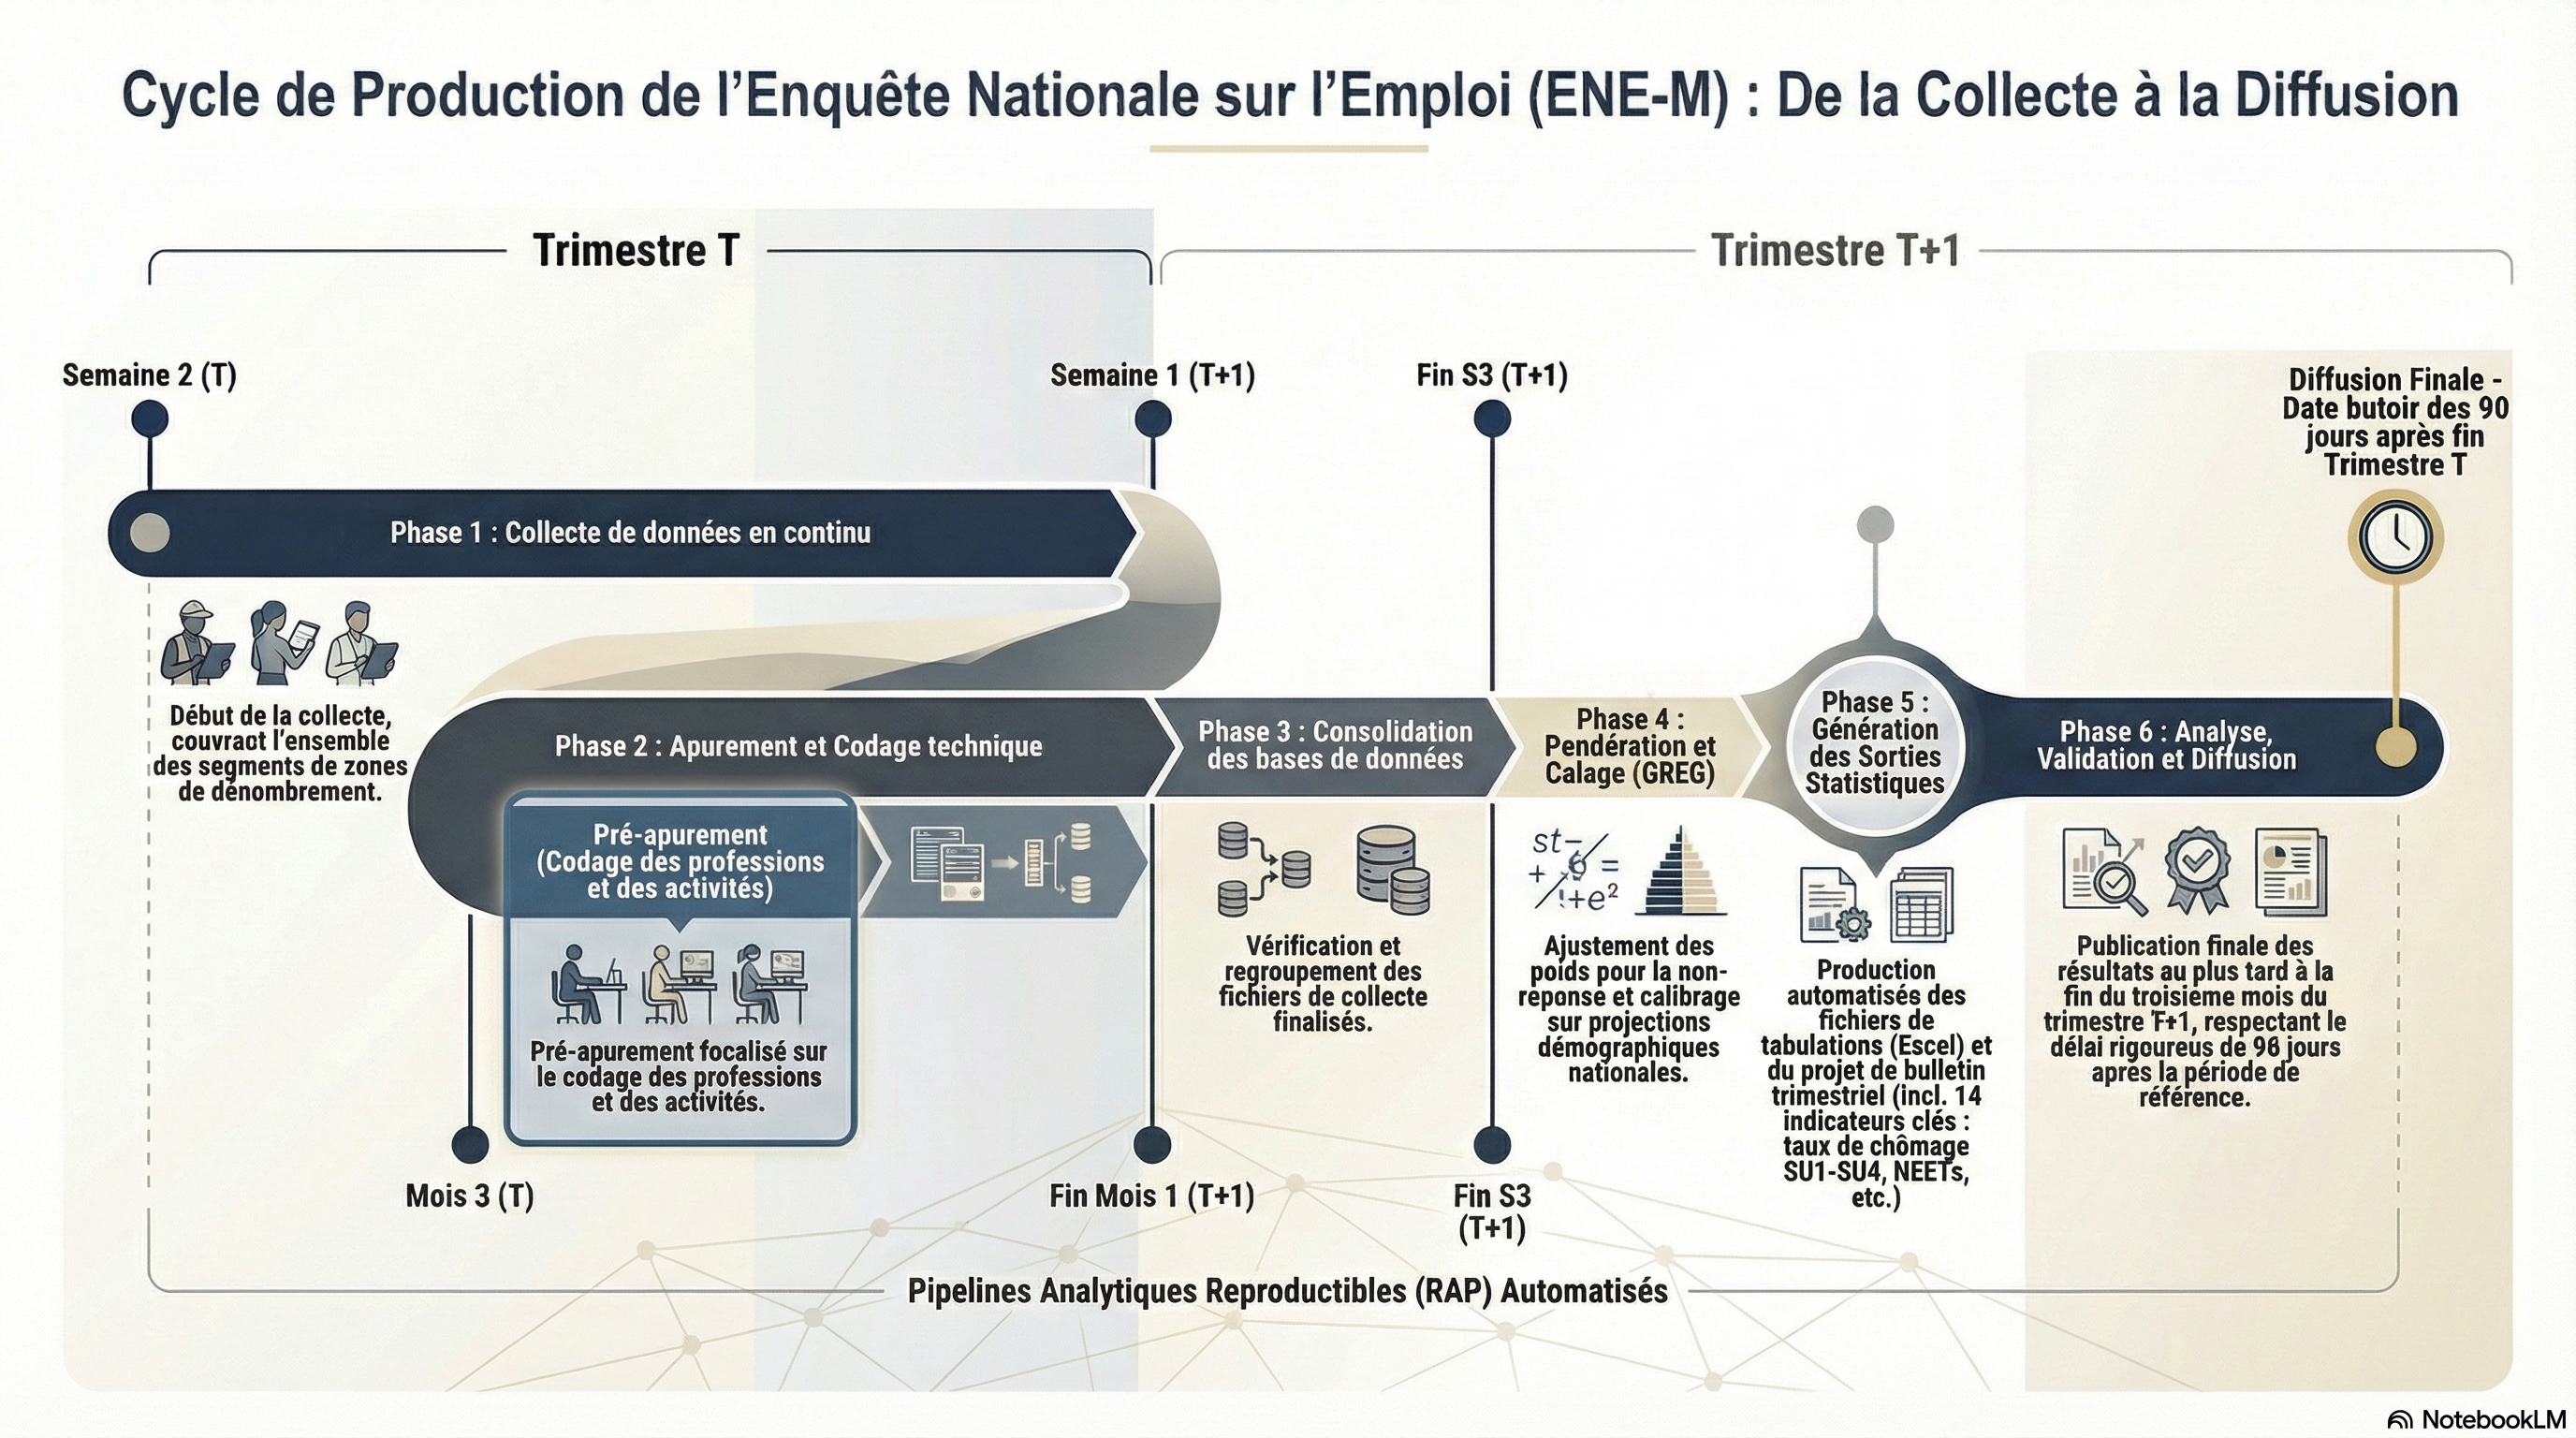
\includegraphics[width=\textwidth]{cycle_production_enem.png}
  \caption{Cycle de production de l'ENE-M : de la collecte à la diffusion}
  \label{fig:cycle_production}
\end{figure}

%% ─── Échantillonnage ─────────────────────────────────────────────────────────
\section{Échantillonnage}

\subsection{Schéma rotatif}

Le caractère rotatif de l'échantillon traduit l'idée selon laquelle un sous-ensemble de l'échantillon sera enquêté à chaque période considérée. On peut dès lors définir un schéma rotatif qui se présente comme la séquence d'entrée et de sortie du ménage de l'échantillon enquêté. La définition du schéma rotatif est fonction de la périodicité considérée par l'échantillon (mensuelle, trimestrielle, semestrielle). Le choix du schéma rotatif est motivé par la précision souhaitée pour l'estimation annuelle des principaux paramètres de l'étude d'une part et par la nature des indicateurs à calculer d'autre part. En effet, cette dernière condition peut s'exprimer suivant diverses approches. Les instituts de statistiques désireux de produire des statistiques mensuellement ou trimestriellement choisiront des schémas de rotation autorisant un chevauchement mensuel ou trimestriel. À titre d'exemple, l'Institut National des Statistiques et des Études Économiques (INSEE) de France a choisi un schéma de rotation « 6\,--\,0 trimestriel » \cite{loonis2009}, les ménages sont intégrés dans l'échantillon sur 6 trimestres et ensuite remplacés par d'autres ménages. Le \textit{Bureau of Labor Statistics} et le \textit{Census Bureau} aux États-Unis utilisent un schéma de rotation « 4\,--\,8\,--\,4 mensuel » \cite{cheng2012}, les ménages intègrent l'échantillon durant les 4 premiers mois, sont sortis durant les 8 mois suivants et réintègrent l'échantillon durant les 4 mois suivants. Le Rwanda a opté pour un schéma de rotation « 1\,--\,1\,--\,1, trimestriel »\footnote{Labour Force Survey Annual Report 2019, \url{https://www.statistics.gov.rw/publication/labour-force-survey-annual-report-2019}}, les ménages sont interrogés sur un premier trimestre, quittent l'échantillon le trimestre suivant, ils sont de nouveau réinterrogés le trimestre d'après, ils quittent l'échantillon au trimestre prochain pour ensuite le réintégrer une dernière fois au trimestre suivant.

Sur la base de ces différentes approches et de nos objectifs, nous avons opté pour un schéma rotatif « 2\,--\,2, trimestriel ». Premièrement, les schémas rotatifs mensuels nécessitent des enquêtes mensuelles qui entraînent des coûts plus élevés. Deuxièmement, le schéma « 6\,--\,0, trimestriel » permet de mesurer les indicateurs de l'emploi trimestriellement et annuellement mais également de mesurer les variations de ces indicateurs trimestriellement et annuellement. Les ménages d'une grappe donnée sont donc enquêtés sur six trimestres consécutifs, ils sont par la suite remplacés par ceux d'une nouvelle grappe du même secteur. Ce procédé entraîne une surutilisation des ménages qui peut entraîner des non-réponses à compter du troisième ou quatrième trimestre. À côté, un schéma rotatif « 1\,--\,1\,--\,1, trimestriel » ne permet pas de mesurer les variations trimestrielles des indicateurs sur les mêmes ménages. À contrario, un schéma rotatif « 2\,--\,2, trimestriel » permet de mesurer les mêmes indicateurs que le schéma rotatif « 6\,--\,0, trimestriel » tout en offrant une meilleure répartition de la charge de l'enquête sur les ménages. Comme illustré par le Tableau~\ref{tab:rotationnel}, à chaque trimestre, un quart (1/4) de l'échantillon est renouvelé.

\bigskip
\begin{table}[H]
\centering
\caption{Disposition Transversale et Longitudinale de l'échantillon}
\label{tab:rotationnel}
\footnotesize
\setlength{\tabcolsep}{4pt}
\begin{tabular}{|l|l|c|c|c|c|c|c|c|c|}
\hline
\multicolumn{10}{|c|}{\textbf{Trimestres d'entrées des ménages dans l'échantillon}} \\
\hline
 & & \textbf{SE A} & \textbf{SE B} & \textbf{SE C} & \textbf{SE D} & \textbf{SE E} & \textbf{SE F} & \textbf{SE G} & \textbf{SE H} \\
\hline
\multirow{14}{*}{\rotatebox{90}{\parbox{5.5cm}{\centering Trimestres d'interrogation des ménages dans l'échantillon}}}
 & T2 2024 & \textbf{A1} & & & & & & & \\
 & T3 2024 & \textbf{A1} & \textbf{B1} & & & & & & \\
 & T4 2024 & & \textbf{B1} & \textbf{C1} & & & & & \\
 & T1 2025 & & & \textbf{C1} & \textbf{D1} & & & & \\
 & T2 2025 & \textbf{A1} & & & \textbf{D1} & \textbf{E1} & & & \\
 & T3 2025 & \textbf{A1} & \textbf{B1} & & & \textbf{E1} & \textbf{F1} & & \\
 & T4 2025 & & \textbf{B1} & \textbf{C1} & & & \textbf{F1} & \textbf{G1} & \\
 & T1 2026 & & & \textbf{C1} & \textbf{D1} & & & \textbf{G1} & \textbf{H1} \\
 & T2 2026 & \textbf{A2} & & & \textbf{D1} & \textbf{E1} & & & \textbf{H1} \\
 & T3 2026 & \textbf{A2} & \textbf{B2} & & & \textbf{E1} & \textbf{F1} & & \\
 & T4 2026 & & \textbf{B2} & \textbf{C2} & & & \textbf{F1} & \textbf{G1} & \\
 & T1 2026 & \textbf{A2} & & \textbf{C2} & \textbf{D2} & & & \textbf{G1} & \textbf{H1} \\
 & T2 2026 & \textbf{A2} & \textbf{B2} & & \textbf{D2} & \textbf{E2} & & & \textbf{H1} \\
 & T3 2026 & & \textbf{B2} & & & \textbf{E2} & \textbf{F2} & & \\
\hline
\end{tabular}
\end{table}

\subsection{Tirage de l'échantillon}

L'échantillon est stratifié par régions administratives ivoiriennes de manière que les résultats annuels soient représentatifs au sein de chaque région. On a donc :
\begin{itemize}[noitemsep]
  \item 56 zones de dénombrement tirées par région à l'exception de la ville d'Abidjan ;
  \item 104 zones de dénombrement tirées dans le district autonome d'Abidjan.
\end{itemize}

Les zones de dénombrement sont tirées à probabilité inégale par rapport à leur taille en individu\footnote{Les tailles en individu proviennent des tailles de population du RGPH 2021.}. On tire alors les cinquante-six (56) zones de dénombrement de la région ou les cent-quatre (104) zones de dénombrement pour le district autonome d'Abidjan en respectant la structure selon les départements, sous-préfectures et le milieu de résidence.

\subsection{Sous-échantillon de zones de dénombrement}

Au sein de chaque région, les zones de dénombrement tirées comme indiqué précédemment sont regroupées en sous-échantillon de zone de dénombrement de manière aléatoire. Dans une région autre que le district d'Abidjan, les cinquante-six (56) zones de dénombrement sont regroupées en huit (8) sous-échantillons chacun contenant sept (7) zones de dénombrement. Au sein du district autonome d'Abidjan, les huit (8) sous-échantillons contiennent treize (13) zones de dénombrement. À chaque trimestre, un sous-échantillon de zones de dénombrement intègre l'échantillon rotatif. Chaque sous-échantillon intégrant est représentatif de la région concernée. La précision des estimations au sein de la région s'améliore avec le temps et l'ajout de sous-échantillons dans l'échantillon global.

\subsection{Segmentation}

Afin de permettre la rotation des ménages selon le schéma susmentionné (cf.\ Tableau~\ref{tab:rotationnel}), un niveau géographique inférieur à la zone de dénombrement a été introduit. Il s'agit d'une subdivision d'une zone de dénombrement selon la répartition des ménages géolocalisées appelée \textbf{segment}. Ainsi, six (6) segments sont construits au sein de chaque zone de dénombrement.

Au sein de chaque ZD intégrant l'échantillon, les segments sont rangés de manière aléatoire de 1 à 6. L'entrée des segments de ZD dans l'échantillon est fonction du rang du segment, du premier au sixième segment. Le Tableau~\ref{tab:repartition} présente l'échantillon trimestriel de l'enquête.

En somme, la sélection des zones de dénombrement est réalisée comme suit :
\begin{enumerate}[label=(\roman*), noitemsep]
  \item Dans cet ensemble de zones de dénombrement, on tire cinquante-six (56) ou cent quatre (104) zones de dénombrement \textbf{selon le milieu de résidence (urbain ou rural)} ;
  \item On subdivise les zones de dénombrement en \textbf{six (6) segments} et on range aléatoirement les segments \textbf{du premier au sixième} ;
  \item Les \textbf{segments de zones de dénombrement intègrent l'échantillon trimestriel} à raison d'un sous-échantillon par trimestre ;
  \item À l'entrée d'un segment, on dénombre l'ensemble des ménages du segment. On tire de manière systématique \textbf{douze (12) ménages} qui seront interrogés.
\end{enumerate}

\bigskip
{\footnotesize
\setlength{\tabcolsep}{3pt}
\begin{longtable}{|>{\centering\arraybackslash}p{3.6cm}|p{3.2cm}|>{\centering\arraybackslash}p{1.0cm}|>{\centering\arraybackslash}p{0.9cm}|>{\centering\arraybackslash}p{1.0cm}|>{\centering\arraybackslash}p{1.5cm}|>{\centering\arraybackslash}p{1.5cm}|}
\caption{Répartition de l'effectif des ménages attendus, du nombre de ZDs à tirer, du nombre de ménages enquêtés trimestriellement}
\label{tab:repartition}\\
\hline
\textbf{DR} & \textbf{Région} & \textbf{Nb SE de ZD} & \textbf{Nb ZD / SE} & \textbf{Nb ZD / région} & \textbf{Nb ménages annuel (1\textsuperscript{re} int.)} & \textbf{Nb ménages trim. (1\textsuperscript{re} int.)} \\
\hline
\endfirsthead
\multicolumn{7}{c}{\tablename~\thetable{} -- suite}\\
\hline
\textbf{DR} & \textbf{Région} & \textbf{Nb SE de ZD} & \textbf{Nb ZD / SE} & \textbf{Nb ZD / région} & \textbf{Nb ménages annuel (1\textsuperscript{re} int.)} & \textbf{Nb ménages trim. (1\textsuperscript{re} int.)} \\
\hline
\endhead
\hline
\endfoot
ABENGOUROU & INDENIE-DJUABLIN & 8 & 7 & 56 & 336 & 84 \\
\hline
ABENGOUROU & SUD-COMOE & 8 & 7 & 56 & 336 & 84 \\
\hline
ABIDJAN & AUTONOME D'ABIDJAN & 8 & 13 & 104 & 624 & 156 \\
\hline
ABIDJAN & GRANDS-PONTS & 8 & 7 & 56 & 336 & 84 \\
\hline
AGBOVILLE & AGNEBY-TIASSA & 8 & 7 & 56 & 336 & 84 \\
\hline
AGBOVILLE & LA ME & 8 & 7 & 56 & 336 & 84 \\
\hline
BONDOUKOU & BOUNKANI & 8 & 7 & 56 & 336 & 84 \\
\hline
BONDOUKOU & GONTOUGO & 8 & 7 & 56 & 336 & 84 \\
\hline
BOUAKE & GBEKE & 8 & 7 & 56 & 336 & 84 \\
\hline
BOUAKE & HAMBOL & 8 & 7 & 56 & 336 & 84 \\
\hline
DALOA & HAUT-SASSANDRA & 8 & 7 & 56 & 336 & 84 \\
\hline
DALOA & MARAHOUE & 8 & 7 & 56 & 336 & 84 \\
\hline
DAOUKRO & IFFOU & 8 & 7 & 56 & 336 & 84 \\
\hline
DAOUKRO & MORONOU & 8 & 7 & 56 & 336 & 84 \\
\hline
GAGNOA & GÔH & 8 & 7 & 56 & 336 & 84 \\
\hline
GAGNOA & LÔH-DJIBOUA & 8 & 7 & 56 & 336 & 84 \\
\hline
KORHOGO & BAGOUE & 8 & 7 & 56 & 336 & 84 \\
\hline
KORHOGO & PORO & 8 & 7 & 56 & 336 & 84 \\
\hline
KORHOGO & TCHOLOGO & 8 & 7 & 56 & 336 & 84 \\
\hline
MAN & CAVALLY & 8 & 7 & 56 & 336 & 84 \\
\hline
MAN & GUEMON & 8 & 7 & 56 & 336 & 84 \\
\hline
MAN & TONKPI & 8 & 7 & 56 & 336 & 84 \\
\hline
ODIENNE & BAFING & 8 & 7 & 56 & 336 & 84 \\
\hline
ODIENNE & FOLON & 8 & 7 & 56 & 336 & 84 \\
\hline
ODIENNE & KABADOUGOU & 8 & 7 & 56 & 336 & 84 \\
\hline
SAN-PEDRO & GBÔKLE & 8 & 7 & 56 & 336 & 84 \\
\hline
SAN-PEDRO & NAWA & 8 & 7 & 56 & 336 & 84 \\
\hline
SAN-PEDRO & SAN-PEDRO & 8 & 7 & 56 & 336 & 84 \\
\hline
SEGUELA & BERE & 8 & 7 & 56 & 336 & 84 \\
\hline
SEGUELA & WORODOUGOU & 8 & 7 & 56 & 336 & 84 \\
\hline
YAMOUSSOUKRO & BELIER & 8 & 7 & 56 & 336 & 84 \\
\hline
YAMOUSSOUKRO & N'ZI & 8 & 7 & 56 & 336 & 84 \\
\hline
YAMOUSSOUKRO & YAMOUSSOUKRO & 8 & 7 & 56 & 336 & 84 \\
\hline
\textbf{Ensemble} & \textbf{Ensemble} & \textbf{264} & \textbf{237} & \textbf{1896} & \textbf{11376} & \textbf{2844} \\
\hline
\end{longtable}
}

%% ─── Déroulement de l'enquête ────────────────────────────────────────────────
\section{Déroulement de l'enquête}

La collecte de l'enquête Emploi volet ménage se caractérise par son principe rotatif trimestriel. Cette approche est l'élément essentiel du changement de méthodologie. Dans le but de bien mesurer les évolutions infra-annuelles, l'enquête est réalisée tout au long de l'année, relativement aux 52 semaines de l'année, les résultats sont présentés trimestriellement et annuellement.

Au sein de chaque région, à l'exception du district d'Abidjan, trois (3) agents enquêteurs dont un chef d'équipe doivent couvrir les sept (7) zones de dénombrement. Au sein de chaque segment, les agents doivent interroger douze (12) ménages sur deux semaines. Les douze (12) ménages du segment sont interrogés relativement à \textbf{deux semaines de référence} à raison de \textbf{six (6) ménages par semaine de référence}. Ainsi, il faudra absolument ne pas réaliser l'interview des douze (12) ménages au cours d'une même semaine à l'exception du District Autonome d'Abidjan. Une zone de dénombrement est interrogée sur \textbf{deux (2) semaines de référence}.

L'affectation des ménages aux semaines de référence est réalisée par tirage aléatoire. La semaine de référence du premier ménage tiré est déterminée par la valeur d'un nombre aléatoire généré entre 0 et 1. Si ce nombre est supérieur ou égal à 0,5, le ménage est associé à la première semaine de référence, si ce nombre est inférieur ou égal à 0,5, le ménage est affecté à la deuxième semaine de référence. Par suite, la semaine de référence du second ménage est systématiquement différente de celle du premier ménage. Ainsi, si le premier ménage est associé à la première semaine, le second sera associé à la deuxième semaine de référence. Pour les autres ménages, tous les ménages de rang impair ont la même semaine de référence que le premier ménage, par analogie, tous les ménages de rang pair ont la même semaine de référence que le second ménage.

Il est fortement recommandé aux enquêteurs de réaliser les entretiens au cours des trois premiers jours de la semaine de collecte afin de :
\begin{enumerate}[label=(\roman*), noitemsep]
  \item Limiter les imprécisions liées aux problèmes de mémoire des enquêtés ;
  \item Dégager du temps pour le ratissage éventuel des ménages des téléopérateurs dans la deuxième semaine d'interrogation de la zone de dénombrement ;
  \item Dégager du temps pour le dénombrement de la prochaine zone de dénombrement avant d'entamer la semaine de référence.
\end{enumerate}

\begin{figure}[H]
  \centering
  \includegraphics[width=\textwidth]{image2.png}
  \caption{Schéma d'interrogation d'un segment d'une zone de dénombrement}
  \label{fig:schema_interrogation}
\end{figure}

\subsection{Le type de questionnaire}

Les ménages sont interrogés sur six trimestres à raison de deux trimestres par an. La nature du questionnaire dépend du rang d'interrogation de l'individu enquêté ou de sa grappe. Le rang traduit l'occurrence d'enquête du ménage, de l'individu ou de la grappe. Le rang de l'individu est très généralement identique au rang de la grappe à laquelle appartient son ménage. Toutefois, il est possible qu'un individu intègre le ménage en cours du processus de collecte. Dans ce cas, il devra répondre au questionnaire de première interrogation. En outre, certaines questions ne sont posées qu'en première interrogation, d'autres ne seront posées que si la situation de l'individu a changé. Le tableau ci-dessous décrit le mécanisme du choix du questionnaire d'entretien selon le rang de l'individu et le rang de la grappe à laquelle appartient son ménage.

\begin{table}[H]
\centering
\caption{Type de questionnaire selon le rang de la grappe et de l'individu}
\label{tab:questionnaire}
\begin{tabular}{|>{\centering\arraybackslash}p{3.9cm}|>{\centering\arraybackslash}p{1.2cm}|>{\centering\arraybackslash}p{2.6cm}|>{\centering\arraybackslash}p{2.6cm}|>{\centering\arraybackslash}p{2.6cm}|}
\hline
\multicolumn{2}{|c|}{} & \multicolumn{3}{c|}{\textbf{Rang de la grappe}} \\
\cline{3-5}
\multicolumn{2}{|c|}{} & \textbf{1} & \textbf{2--5} & \textbf{6} \\
\hline
\multirow{3}{3.9cm}{\centering\textbf{Rang de l'individu}} & \textbf{1} & 1\textsuperscript{ère} interrogation & 1\textsuperscript{ère} interrogation & 1\textsuperscript{ère} interrogation \\
\cline{2-5}
 & \textbf{2--5} & & 2\textsuperscript{ème} à 5\textsuperscript{ème} interrogation & 6\textsuperscript{ème} interrogation \\
\cline{2-5}
 & \textbf{6} & & & 6\textsuperscript{ème} interrogation \\
\hline
\end{tabular}
\end{table}

\subsection{Le mode d'interrogation}

Le mode d'interrogation est fonction du rang de l'individu. Comme dans le cas de la nature du questionnaire, le rang de l'individu est généralement identique au rang de la grappe sauf dans le cas où l'individu intègre le ménage au cours du processus de collecte.

Ainsi, la première interrogation est réalisée en entretien face-à-face. Les vagues suivantes sont réalisées par appel téléphonique dans l'objectif de réduire les coûts de collecte. Toutefois, après dix (10) tentatives téléphoniques infructueuses, l'agent de terrain devra interroger les individus en entretien face-à-face.

%% ─── Outils de collecte ──────────────────────────────────────────────────────
\section{Outils de Collecte}

Les outils de collecte sont constitués de l'ensemble des documents techniques devant servir à la réalisation efficiente de la collecte des informations sur le terrain. Pour l'Enquête Emploi Continue, comme présenté à la section \textit{Déroulement de l'enquête}, le type de questionnaire dépend du rang de l'individu et du rang de la grappe à laquelle appartient le ménage de l'individu.

\subsubsection*{Questionnaire ménage}

Il permet de dresser la liste de tous les membres des ménages, de collecter des informations sur leurs caractéristiques sociodémographiques de base (lien de parenté, âge, sexe, niveau d'instruction, situation matrimoniale, etc.). Il permet également de collecter des données sur les commodités du logement et les caractéristiques socio-économiques du ménage. Le questionnaire ménage permet également de déterminer les personnes éligibles au questionnaire individuel.

\subsubsection*{Questionnaire individuel}

Il comprend les sections suivantes :
\begin{itemize}[noitemsep]
  \item Autres Formes de Travail ;
  \item Situation d'emploi ;
  \item Emploi principal ;
  \item Emploi secondaire ;
  \item Compétences et qualifications requises pour l'emploi principal ;
  \item Pluriactivité ;
  \item Emploi Secondaire ;
  \item Temps de travail ;
  \item Situations d'emploi inadéquates ;
  \item Recherche d'emploi et disponibilités ;
  \item Chômage ;
  \item Emploi Antérieur ;
  \item Insertion Professionnelle des diplômés ;
  \item Revenu Hors Emploi ;
  \item Activité des Parents ;
  \item Disponibilité des individus.
\end{itemize}

À chaque trimestre, des modules complémentaires peuvent être intégrés au questionnaire principal. En 2025, il est prévu l'intégration d'un module sur le travail domestique et un module sur le travail des enfants.

%% ─── Pondération et Précision ────────────────────────────────────────────────
\section{Pondération et Précision de l'enquête}

\subsection{Pondération de l'enquête}

Le schéma de l'enquête met en évidence deux types de pondération : une pondération transversale et une pondération longitudinale. La pondération transversale se définit comme la pondération affectée à un individu lors de l'estimation d'un indicateur transversal (taux de chômage trimestriel, nombre de demandeurs d'emploi trimestriel, etc.). La pondération longitudinale se définit comme la pondération affectée à un individu lors de l'estimation d'un indicateur de transition (changement de statut dans l'emploi d'un individu entre deux trimestres). La pondération étant l'inverse de la probabilité d'inclusion, par la suite nous présenterons les probabilités d'inclusion des zones de dénombrement et des ménages.

\subsubsection{Probabilité d'inclusion d'une zone de dénombrement}

\begin{equation}
  \pi_{ZD} = k \times \dfrac{N_{men\_ZD}}{N_{men\_strat}} \times \dfrac{N_{ZD\_strat}}{k}
           = \dfrac{N_{men\_ZD}}{N_{men\_strat}} \times N_{ZD\_strat}
\end{equation}

avec $N_{men\_ZD} \approx N_{men\_segment} \times 6$, et :
\begin{itemize}[noitemsep]
  \item \textbf{Si Abidjan} ($k = 104$) :
    $\displaystyle\pi_{ZD} = 104 \times \dfrac{N_{men\_ZD}}{N_{men\_strat}} \times \dfrac{N_{ZD\_strat}}{104}$
  \item \textbf{Si autre région} ($k = 56$) :
    $\displaystyle\pi_{ZD} = 56 \times \dfrac{N_{men\_ZD}}{N_{men\_strat}} \times \dfrac{N_{ZD\_strat}}{56}$
\end{itemize}

Avec :
\begin{itemize}[noitemsep]
  \item $N_{men\_ZD}$ : nombre estimé de ménages dans la ZD (calculé comme $N_{men\_segment} \times 6$) ;
  \item $N_{men\_strat}$ : nombre total de ménages dans la strate (région) ;
  \item $N_{ZD\_strat}$ : nombre total de zones de dénombrement dans la strate.
\end{itemize}

\subsubsection{Probabilité d'inclusion d'un ménage dans une zone de dénombrement (pondération transversale)}

Dans le cadre de la pondération transversale, la probabilité d'inclusion d'un ménage est calculée de manière identique quelle que soit son occurrence d'interrogation (première interrogation ou ré-interrogation). Elle repose sur les paramètres du plan de sondage et non sur les réalisations effectives :

\begin{equation}
  \pi_{men} = \frac{n_{cible}}{N_{denomb\_segment}} \times \frac{1}{6}
\end{equation}

Avec :
\begin{itemize}[noitemsep]
  \item $n_{cible} = 12$ : nombre de ménages cible à enquêter par segment (constante de design) ;
  \item $N_{denomb\_segment}$ : nombre total de ménages dénombrés dans le segment ;
  \item $1/6$ : probabilité de sélection du segment parmi les six segments de la ZD.
\end{itemize}

L'écart entre $n_{cible}$ et le nombre de ménages réellement enquêtés est pris en charge par le facteur d'ajustement pour non-réponse appliqué à l'étape suivante.

\subsection{Ajustement pour la non-réponse}

Entre le poids de base et la calibration, un ajustement intermédiaire est appliqué pour compenser la non-réponse totale des ménages. Lorsqu'un ménage tiré dans l'échantillon ne peut être enquêté (refus, absence prolongée, logement vide), le poids des ménages répondants du même groupe est majoré afin de préserver la représentativité de l'échantillon. Le facteur d'ajustement est calculé par groupe homogène (Région $\times$ Milieu) :

\begin{equation}
  f_{NR} = \frac{n_{théorique}}{n_{répondants}}
\end{equation}

où $n_{théorique}$ désigne le potentiel de collecte théorique du groupe (cible de 12 ménages par segment, plafonnée au nombre dénombré) et $n_{répondants}$ le nombre de ménages ayant effectivement répondu. Le poids ajusté pour la non-réponse est alors :

\begin{equation}
  w^{(1)}_i = w^{(0)}_i \times f_{NR}
\end{equation}

Ce poids $w^{(1)}$ constitue l'entrée du processus de calibration.

\subsection{Calibration (Calage)}

\subsubsection{Principe et objectif}

La calibration constitue la dernière étape d'ajustement des poids avant la production des estimations. Elle vise à assurer la cohérence des estimations pondérées avec des totaux de population connus issus de sources externes fiables — en l'occurrence les projections démographiques établies à partir du Recensement Général de la Population et de l'Habitat (RGPH 2021). Formellement, le calage consiste à trouver de nouveaux poids $w_{final}$ proches des poids initiaux $w^{(1)}$ tels que :

\begin{equation}
  \sum_{i \in \mathcal{S}} w_{final,i} \cdot \mathbf{x}_i = \mathbf{T}_X
\end{equation}

où $\mathbf{x}_i$ est le vecteur des variables auxiliaires de l'individu $i$ (sexe, âge, milieu de résidence, région) et $\mathbf{T}_X$ le vecteur des totaux de population correspondants. La méthode retenue est l'estimateur par régression généralisée (GREG) implémenté dans le package R \texttt{ReGenesees} \cite{zardetto2015}, avec une fonction de distance de type \textit{logit} permettant de contraindre les facteurs de correction dans des bornes prédéfinies et d'éviter ainsi des poids extrêmes ou négatifs.

\subsubsection{Structure des contraintes de calage}

Le schéma de référence retenu pour la pondération trimestrielle est le schéma \textbf{180X\_1D}, comportant 180 contraintes définies sur un domaine national unique. Ces contraintes sont organisées en deux niveaux géographiques :

\begin{itemize}[noitemsep]
  \item \textbf{Niveau national ($X_1$--$X_{48}$) :} 48 contraintes croisant le sexe (homme/femme), le milieu de résidence (urbain/rural) et 12 groupes d'âge quinquennaux (de 0--4 ans à 65 ans et plus). Ces contraintes assurent l'alignement des estimations sur la structure démographique nationale fine.
  \item \textbf{Niveau régional ($X_{49}$--$X_{180}$) :} 132 contraintes réparties sur les 33 régions administratives de Côte d'Ivoire, à raison de 4 contraintes par région croisant le sexe et deux groupes d'âge larges (0--14 ans et 15 ans et plus). Ces contraintes garantissent la représentativité régionale des estimations.
\end{itemize}

Pour chaque contrainte $k$, une variable indicatrice $\mathbf{1}_{[i \in C_k]}$ est construite dans les données d'échantillon, et le total de population correspondant $T_k$ est extrait des projections démographiques. Le système de 180 équations ainsi constitué est résolu simultanément par le calage.

\subsubsection{Mise en \oe{}uvre avec ReGenesees}

La procédure de calibration est orchestrée en sept étapes séquentielles :

\begin{enumerate}[label=(\roman*), noitemsep]
  \item Chargement des données d'enquête et des totaux de population de référence ;
  \item Construction des variables indicatrices de contrainte ($X_1$ à $X_{180}$) dans les données d'échantillon ;
  \item Construction des totaux de population correspondants à partir des projections du RGPH 2021 ;
  \item Création de l'objet de plan de sondage \texttt{ReGenesees} : plan stratifié à deux degrés (ZD puis ménage), avec \texttt{ids = \textasciitilde PSUKEY + HHKEY}, \texttt{strata = \textasciitilde STRATAKEY} et \texttt{weights = \textasciitilde d\_weights} ;
  \item Exécution du calage par la méthode \textit{logit}, avec application de bornes $[l,\, u]$ sur les facteurs de correction $g_i$ ;
  \item Attachement des poids calibrés au fichier individuel complet ;
  \item Calcul des indicateurs de précision post-calage (coefficients de variation par domaine).
\end{enumerate}

Le poids final de chaque individu est obtenu comme le produit de son poids d'entrée et du facteur de correction issu du calage :

\begin{equation}
  w_{final,i} = g_i \times w^{(1)}_i
\end{equation}

où $g_i$ (\texttt{FINAL\_CORR\_FACTOR}) est contraint par la méthode logit à demeurer dans un intervalle $[l, u]$ garantissant l'absence de poids nuls ou excessifs.

Le schéma retenu pour la production des estimations trimestrielles standard est le schéma \textbf{180X\_1D}, comportant 180 contraintes définies sur un domaine national unique.

\subsection{Pondération longitudinale et correction de l'attrition}

La pondération longitudinale est utilisée pour l'estimation d'indicateurs de transition (ex. : changement de statut dans l'emploi entre deux trimestres). Elle est construite à partir des poids \textbf{calibrés transversaux} $w_{final}$, auxquels est appliqué un facteur correctif de l'attrition estimé par régression logistique :

\begin{equation}
  w_{long,i} = w_{final,i} \times \frac{1}{\hat{p}_{attrition,i}}
\end{equation}

où $\hat{p}_{attrition,i}$ est la probabilité estimée qu'un individu $i$ soit présent à la ré-interrogation, modélisée par régression logistique sur des variables observables (caractéristiques sociodémographiques du ménage et de l'individu au trimestre de première interrogation). Cette construction garantit que le poids longitudinal hérite de la cohérence démographique assurée par la calibration transversale.

\subsection{Précision et Calcul de Variance}

\subsubsection{Précision}

La précision de l'enquête Emploi continue est tributaire d'erreur d'estimations mesurées par l'écart-type de chaque estimation, les estimations de ces erreurs sont fonction du plan de sondage et des procédures de post-stratification. La variable d'intérêt principale retenue est le taux combiné du chômage et de la main-d'\oe{}uvre potentielle (SU3). Considérant les effectifs de ménages attendus (cf.\ Tableau~\ref{tab:repartition}), au premier trimestre d'interrogation l'estimation du SU3 est réalisée dans un intervalle de confiance à 95\,\% de $\pm1{,}67$ points de pourcentage sur l'étendue du territoire pour un niveau de précision de 0,00853117. La précision de l'estimation s'améliore avec le temps à mesure que des sous-échantillons de zone de dénombrement intègrent l'échantillon. En régime de croisière, en absence d'attrition, l'estimation du SU3 est réalisée dans un intervalle de confiance à 95\,\% de $\pm0{,}84$ points de pourcentage sur l'étendue du territoire pour un niveau de précision de 0,0042655. Le schéma rotatif de l'échantillon doit permettre d'obtenir une meilleure précision des estimateurs annuels obtenus par cumul des échantillons trimestriels.

Il convient de noter que l'hypothèse d'absence d'attrition permet d'obtenir une égalité entre le nombre de ménages enquêtés annuellement en première interrogation et le nombre de ménages enquêtés trimestriellement en première interrogation ou plus. Il faudra remarquer que l'hypothèse d'absence d'attrition étant difficile à valider dans le temps, il est naturel de penser qu'au fil des trimestres, le nombre de ménages enquêtés trimestriellement en régime de croisière soit inférieur au nombre de ménages enquêtés chaque année en première interrogation. La différence viendrait du nombre de ménages non retrouvés ou injoignables en ré-interrogation.

\begin{table}[H]
\centering
\caption{Précision des estimations en point de pourcentage (intervalle de confiance à 95\,\%)}
\label{tab:precision}
\footnotesize
\begin{tabular}{lccc}
\toprule
 & \textbf{Trimestrielle} & \multicolumn{2}{c}{\textbf{Annuelle}} \\
\cmidrule(lr){3-4}
 & \textbf{(régime de croisière)} & \textbf{1\textsuperscript{re} int. uniquement} & \textbf{Tous ménages (approx.)} \\
\midrule
Abidjan        & $\pm3{,}57$ & $\pm3{,}57$  & $\approx\pm1{,}79$ \\
Autres Régions & $\pm4{,}86$ & $\pm4{,}86$  & $\approx\pm2{,}43$ \\
Côte d'Ivoire  & $\pm0{,}84$ & $\pm0{,}48$  & $\approx\pm0{,}42$ \\
\bottomrule
\end{tabular}
\end{table}

\noindent\textit{Notes : (1) La colonne « 1\textsuperscript{re} int. uniquement » cumule les ménages en première interrogation sur les quatre trimestres de l'année. Pour Abidjan et les autres régions, l'effectif annuel ainsi constitué est équivalent à l'effectif trimestriel en régime de croisière (tous ménages confondus), ce qui explique l'égalité des valeurs entre les deux premières colonnes pour ces domaines. (2) La colonne « Tous ménages » est une approximation supposant que l'utilisation de l'ensemble des ménages enquêtés sur l'année (premières et ré-interrogations) divise la variance par 4, soit un intervalle de confiance approximativement divisé par 2.}

\subsubsection{Estimation d'une moyenne annuelle des indicateurs}

Une estimation annuelle se définit comme la combinaison des estimations trimestrielles en prenant en compte tous les individus en première ou seconde interrogation à tous les trimestres de l'année. Nous recherchons donc la combinaison des estimations trimestrielles qui permet d'obtenir une estimation sans biais de variance minimale.

Soit $\widehat{\theta}_{i}^{j}$, l'estimateur sans biais du paramètre $\theta$ pour le trimestre $i$ pour l'année $j$, avec $i \in \llbracket 1,4 \rrbracket$. Soit $\widehat{\theta}^{j}$, l'estimateur du paramètre $\theta$, pour une année $j$. On définit $\widehat{\theta}$ comme suit :

\begin{equation}
  \widehat{\theta}^{j} = \sum_{i=1}^{4} \alpha_{i}\, \widehat{\theta}_{i}^{j}
\end{equation}

Dans le but de déterminer les valeurs $\alpha_{i}$, il faut déterminer l'estimateur de variance minimale. La variance de l'estimateur $\widehat{\theta}^{j}$ s'écrit comme suit :

\begin{equation}
  V\!\left(\widehat{\theta}^{j}\right) = \sum_{i=1}^{4} \alpha_{i}^{2}\, V\!\left(\widehat{\theta}_{i}^{j}\right)
\end{equation}

Le calcul des paramètres $\alpha_{i}$ nécessite la minimisation de la variance de l'estimateur $\widehat{\theta}^{j}$, on résout donc le programme suivant :

\begin{equation}
  \left\{
  \begin{aligned}
    &\min_{\alpha_1,\alpha_2,\alpha_3,\alpha_4} \sum_{i=1}^{4} \alpha_{i}^{2}\, V(\theta_{i}) \\
    &\text{s/c} \quad \sum_{i=1}^{4} \alpha_{i} = 1
  \end{aligned}
  \right.
\end{equation}

La solution du programme est $\{\alpha_1,\alpha_2,\alpha_3,\alpha_4\}$ tel que :

\begin{equation}
  \alpha_{i} = \frac{\displaystyle\sum_{\substack{j=1 \\ j \neq i}}^{4} V(\theta_{j})}
  {V(\theta_1)V(\theta_2)V(\theta_3) + V(\theta_1)V(\theta_2)V(\theta_4) + V(\theta_1)V(\theta_3)V(\theta_4) + V(\theta_2)V(\theta_3)V(\theta_4)}
\end{equation}

En pratique, l'approche directe est retenue : $\alpha_{i} = \frac{1}{K}\ \forall\, i \in \{1,\ldots,K\}$, où $K \leq 4$ désigne le nombre de trimestres disponibles pour l'année considérée. Cette approche se traduit, au niveau des poids individuels, par :

\begin{equation}
  w_{annuel,i} = \frac{w_{final,i}}{K}
\end{equation}

où $w_{final,i}$ désigne le poids calibré (\texttt{FINAL\_WEIGHT}) de l'individu $i$ au trimestre $t$. Le fichier annuel est obtenu par empilement (\textit{bind\_rows}) des fichiers trimestriels calibrés, la valeur de $K$ étant détectée automatiquement en fonction des fichiers disponibles.

%% ─── Diffusion des résultats ─────────────────────────────────────────────────
\section{Diffusion des Résultats}

\subsection{Calendrier de publication}

Conformément aux recommandations de la Conférence Internationale des Statisticiens du Travail (CIST), les résultats de chaque trimestre sont publiés dans un délai maximum de \textbf{90 jours} après la fin de la période de référence. Ce délai couvre les phases de collecte, de traitement des données, de calcul des pondérations, de production des indicateurs et de validation des résultats avant diffusion.

\subsection{Indicateurs produits}

L'enquête produit trimestriellement et annuellement quatorze indicateurs clés du marché du travail, conformes aux normes de l'Organisation Internationale du Travail (OIT) :

\begin{itemize}[noitemsep]
  \item \textbf{Population en Âge de Travailler (PAT)} : ensemble des individus âgés de 16 ans et plus ;
  \item \textbf{Taux d'emploi} : proportion de personnes en emploi au sein de la PAT ;
  \item \textbf{Taux de chômage (SU1)} : chômage au sens strict du BIT ;
  \item \textbf{SU2} : chômage élargi au sous-emploi lié au temps de travail ;
  \item \textbf{SU3} : chômage élargi à la main-d'\oe{}uvre potentielle (indicateur de référence de l'enquête) ;
  \item \textbf{SU4} : mesure composite de la sous-utilisation de la main-d'\oe{}uvre ($\text{SU2} + \text{SU3} - \text{SU1}$) ;
  \item \textbf{Emploi vulnérable} : travailleurs indépendants et aides familiaux ;
  \item \textbf{Emploi précaire} : emplois temporaires et informels ;
  \item \textbf{Informalité} : part de l'emploi informel selon la Classification Internationale de la Situation dans l'Emploi (CISE-18) ;
  \item \textbf{Classification CISE-18} : répartition de l'emploi selon les statuts définis par la 18\textsuperscript{e} CIST ;
  \item \textbf{NEETs} : proportion de jeunes ni en emploi, ni en éducation, ni en formation ;
  \item \textbf{Branches d'activité} : répartition de l'emploi selon les branches d'activité économique.
\end{itemize}

\subsection{Supports de diffusion}

Pour chaque trimestre, deux livrables sont produits de manière systématique :

\begin{enumerate}[label=(\roman*), noitemsep]
  \item Un \textbf{fichier de tabulations} (\texttt{Tableaux\_Indicateurs\_ENEM.xlsx}) regroupant l'ensemble des tableaux statistiques des indicateurs, ventilés par région, milieu de résidence, sexe et groupe d'âge ;
  \item Un \textbf{bulletin trimestriel} (\texttt{bulletin\_T\{X\}\_\{YYYY\}.docx}) présentant une synthèse analytique des principaux résultats du marché du travail, accompagnée de visualisations graphiques.
\end{enumerate}

\subsection{Approche de production : Pipelines Analytiques Reproductibles}

La production de ces livrables repose sur une approche de \textbf{Pipelines Analytiques Reproductibles} (\textit{Reproducible Analytical Pipelines}, RAP). Cette démarche, adoptée par plusieurs instituts nationaux de statistique, garantit que l'intégralité du processus — du traitement des données brutes à la génération du bulletin — est automatisée, documentée et versionnée sous contrôle de source (Git).

Le pipeline de production comprend quatre étapes automatisées :
\begin{enumerate}[label=(\roman*), noitemsep]
  \item Chargement et préparation des données d'enquête pondérées ;
  \item Calcul des indicateurs du marché du travail et génération des tableaux de résultats ;
  \item Validation automatique de la cohérence des indicateurs (7 tests) ;
  \item Rendu du bulletin trimestriel à partir d'un document source \texttt{Quarto} (\texttt{.qmd}).
\end{enumerate}

Cette approche assure la \textbf{traçabilité} des résultats, leur \textbf{reproductibilité} d'un trimestre à l'autre, et facilite la \textbf{mise à jour} du bulletin lors de l'intégration d'un nouveau trimestre.

%% ─── Références ──────────────────────────────────────────────────────────────
\newpage
\begin{thebibliography}{9}
\bibitem{loonis2009}
Loonis, V. (2009).
\textit{La construction du nouvel échantillon de l'Enquête Emploi en Continu à partir des fichiers de la Taxe d'Habitation}.
JMS, 2009, 23.

\bibitem{cheng2012}
Cheng, Y. (2012).
Overview of current population survey methodology.
In \textit{Proceedings of the Survey Research Methods Section}.
Washington, DC: American Statistical Association (pp. 3963--3979).

\bibitem{zardetto2015}
Zardetto, D. (2015).
ReGenesees: an Advanced R System for Calibration, Estimation and Sampling Error Assessment in Complex Sample Surveys.
\textit{Journal of Official Statistics}, 31(2), 177--203.
\url{https://www.istat.it/en/classifications-and-tools/methods-and-software-of-the-statistical-process/process-phase/weighting-estimation-and-sampling-error-evaluation/regenesees/}
\end{thebibliography}

\end{document}
